In this chapter, 

\section{Flow}

In this section, the general flow of the usage of the visualization application is guided. At the beginning, the blockchain system is empty, and the user can either upload a configuration file or add nodes manually (Figure \ref{fig:start of the application}). The introduction starts with creating nodes and publishing transactions manually, as it is clearer to begin with an simple example.

\begin{figure}[htb]
    \centering
    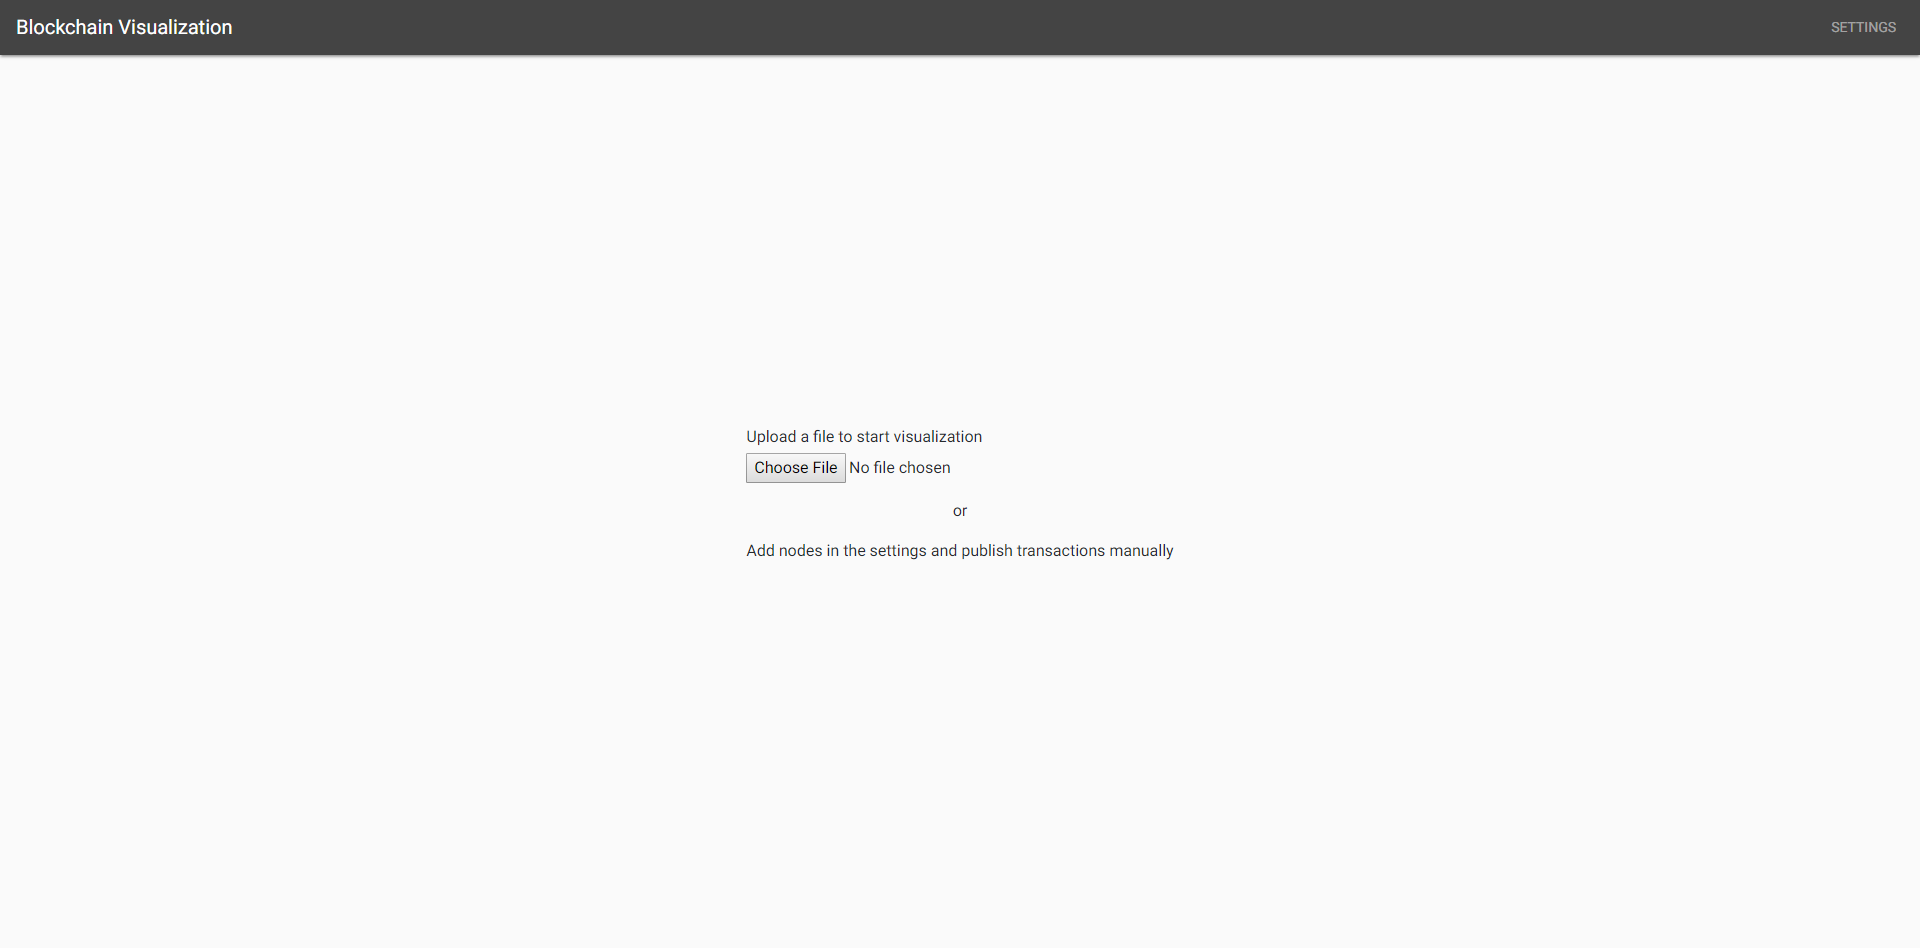
\includegraphics[width=\textwidth]{application_start}
    \caption{Start of the Application.}
    \label{fig:start of the application}
\end{figure}

By clicking the top right button in the navigation bar, the user will be redirected to the settings page, as Figure \ref{fig:settings page} shows.

\begin{figure}[htb]
    \centering
    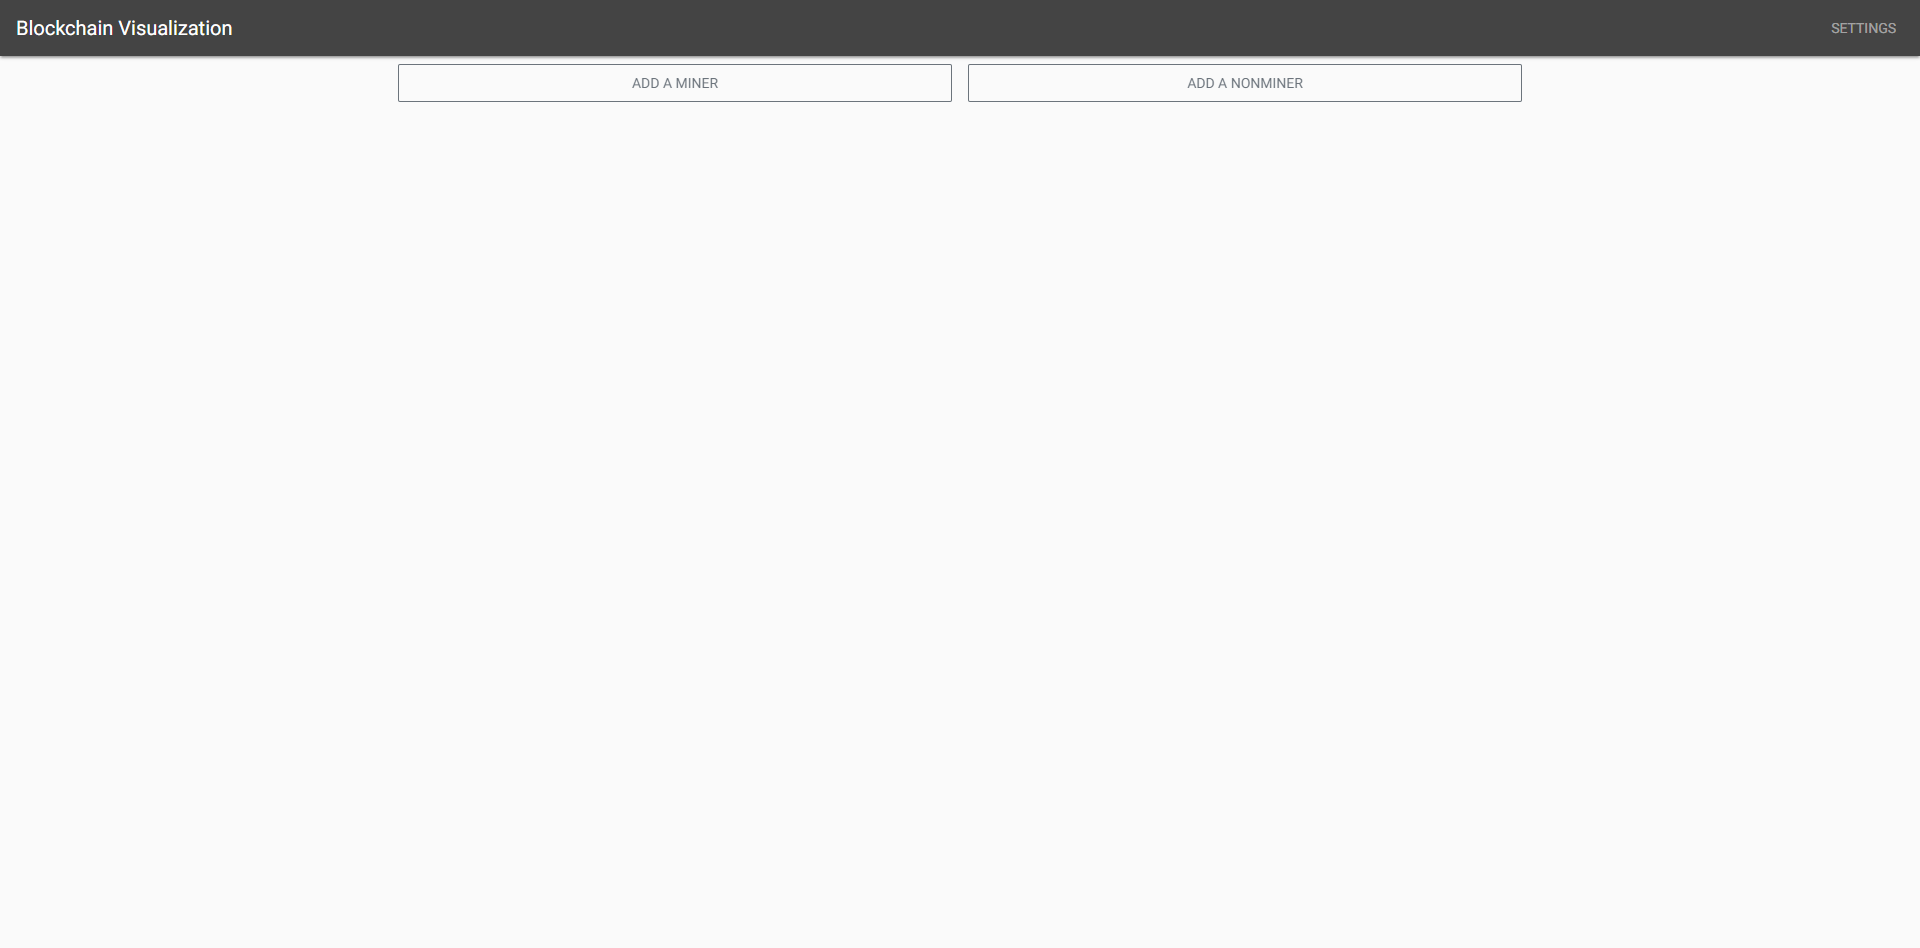
\includegraphics[width=\textwidth]{application_settings1}
    \caption{Settings Page.}
    \label{fig:settings page}
\end{figure}

The settings page contains all the nodes that exist on the blockchain network. However, the blockchain system is empty currently, so the settings page is empty. To add a node, the user can click ``ADD A MINER'' button or ``ADD A NONMINER'' button. In this example, we add three miners and two nonminers.

\section{Configuration Files}

To replay the same visualization of blockchain processes, we can define the configuration of the blockchain system in a file and upload it to the application. The configuration file is composed of three parts: the properties and the parameters of mining strategies of nodes, the delays of networks between each node, and the transactions that will be published through the network. The file is in JSON format, and the file is uploaded to initialize the blockchain system at the beginning.

First, for nodes, it is important to define a unique transaction generator at first, and then it is followed by miners and nonminers. After that, a list of delays between each node is defined. As mentioned before, the transaction generator only connects to miners, and miners and nonminers connect with each other. In the last part, it contains a list of transactions with rewards and the time when the transaction will be published after the starting of the blockchain system.